\documentclass{article}
\usepackage[utf8]{inputenc}
\usepackage{amsmath,amssymb,amsfonts,amsthm}
\usepackage[shortlabels]{enumitem}
\usepackage{etoolbox}
\usepackage{graphicx}
\usepackage{hyperref}


\theoremstyle{plain}
\newtheorem{theorem}{Theorem}
\newtheorem{corollary}[]{Corollary}
\newtheorem{lemma}[]{Lemma}
\newtheorem{proposition}[]{Proposition}
\theoremstyle{definition}
\newtheorem{definition}[]{Definition}
\newtheorem{example}[]{Example}
\newtheorem{conjecture}[]{Conjecture}
\newtheorem{assumption}[]{Assumption}
\newtheorem{claim}[]{Claim}
\newtheorem{rule2}[]{Rule}
\theoremstyle{remark}
\newtheorem{remark}[]{Remark}

\usepackage{color}

\newtoggle{DEBUG}
\toggletrue{DEBUG}
%\togglefalse{DEBUG}


\iftoggle{DEBUG}{
    \newcommand{\michaels}[1]{{\color{blue}#1 (Michael)}}
    \newcommand{\shaide}[1]{{\color{green}#1 (Shai)}}
}{
    \newcommand{\michaels}[1]{}
    \newcommand{\shaide}[1]{}
}

\title{Prunality of the GHOSTDAG Protocol}
\author{Michael Sutton, Shai Wyborski}
\date{July 2020}

\newcommand{\score}[1]{{w\bigl(#1\bigr)}}
\newcommand{\argmax}[2]{\mbox{argmax}_{#1}\{#2\}}
\newcommand{\virt}{\mbox{Virtual}}

\newcommand{\comma}[2]{
    \begin{aligned}#1 & : & #2\end{aligned}
}

\begin{document}

\maketitle

\section{Introduction}

This document details a set of rules miners in the GHOSTDAG \cite{sompolinsky2018phantom} protocol must follow in order to support secure pruning of the DAG.

\section{Notation and Rules}

Parameters:
\begin{itemize}
    \item $\phi$ -- Finality depth
    \item $k$ -- PHANTOM parameter
    \item $\ell$ -- Merge bound
    \item $\pi = 2\phi + 4 \ell k + 2k + 2$ -- Pruning depth
\end{itemize}

\begin{definition}
    Some notations:
    \begin{itemize}
        \item $\overline{P}ast, \overline{F}uture, \overline{C}hain$ are the inclusive counterparts of $Past, Future, Chain$
        % \item $\min, \max$ operators applied to blocks reflect topological relations: $C < B \Rightarrow C \in B.Past$
        % \item $B \vee C = \max B.Chain \cap C.Chain$
        \item $B.Subtree = \{ \comma{C}{B \in C.Chain} \}$
        \item $B.MergeSet = B.Past \setminus B.SelectedParent.\overline{P}ast$  
        \item A block $B$ is said to be a \emph{merging block} of block $Y$, if $Y \in B.MergeSet$.
    \end{itemize}
\end{definition}

\begin{definition} \label{def:blue_depth}
    For any integer $n$ and any block $B$ let $$B_n = \argmax{C\in B.Chain}{\score{C} < \score{B} - n};$$ 
    
    We name some useful blocks:
    \begin{itemize}
        \item The block at \emph{depth} $n$  is $\virt_n$
        \item The \emph{finality block} is $F = \virt_\phi$
        \item The \emph{pruning block} is $P = \virt_\pi$
    \end{itemize}
\end{definition}

\begin{corollary} \label{corollary:depth_bounds}
    For any integer $n$ and any block $B$ $$\score{B} - n - k - 1 \le \score{B_n} < \score{B} - n;$$
\end{corollary}
\begin{proof}
    The second inequality follows directly from Definition \ref{def:blue_depth}. The first follows from maximality of $B_n$. Assume $\score{B_n} < \score{B} - n - k - 1$. Since each chain block can add at most $k+1$ blue blocks, their must exist a block $C \in B.Chain$ where $C.SelectedParent = B_n$, and which satisfies $ \score{C} < \score{B} - n$. Contradicting maximality of $B_n$.
\end{proof}

\begin{corollary} \label{corollary:depth_relation}
    For any block $B$ and any integers $m, n$ s.t. $m>n$ $$\score{B_m} < \score{B_n}+n+k+1 - m;$$
\end{corollary}
\begin{proof}
    This is a direct result of applying Corollary \ref{corollary:depth_bounds} over $B, m$ and obtaining $\score{B_m} < \score{B} - m$, applying the same corollary over $B, n$ and obtaining $\score{B}-n-k-1 \le \score{B_n}$, and combining the inequalities. 
\end{proof}


\begin{definition}[Pruning invalidation rules]
    A block $B$ is considered invalid if one of the following holds:
    \begin{enumerate}[(R-I)]
        \item (Objective finality) 
        % $$\comma{\exists Y \in B.MergeSet \cap B_\phi.Anticone}{Y.Future \cap B.Blues \cap B_\phi.Subtree = \emptyset}$$ 
        \begin{align*}
            \exists Y \in B.MergeSet & \cap B_\phi.Anticone:  \\
            & Y.Future \cap B.Blues \cap B_\phi.Subtree = \emptyset
        \end{align*}
        \label{inv_fin}
        \item (Bounded merge) $$|B.MergeSet| > \ell$$ \label{inv_merge}
        \item (Blood exile) $$\comma{\exists C \in B.Parents}{C\mbox{ is invalid}} $$\label{inv_inh}
    \end{enumerate}
\end{definition}

\begin{assumption} \label{bounded_reorg}
    There is no 51\% attacker and $\phi$ was chosen so that (malicious or organic) splits of depth $\phi$ have negligible probability. We consider them as impossible.
\end{assumption}

\section{Main Proposition}

\begin{proposition}\label{pruning}
   If when $B$ was discovered it held that $B\notin P.Future$ then $B$ will never be in the past of $\virt$.
\end{proposition}

\begin{proof}
    Let $Y$ be a block which, when it was discovered, was not in $P.Future$. Assume that at some future point in time $Y$ was in $\virt.Past$. Let $X\in \virt.Past$ be minimal such that $F\in X.Chain$ and $Y\in X.Past$, such an $X$ must exist by hypothesis and Assumption \ref{bounded_reorg} (though it may not be unique).
    
    \begin{figure}[h]
        \centering
        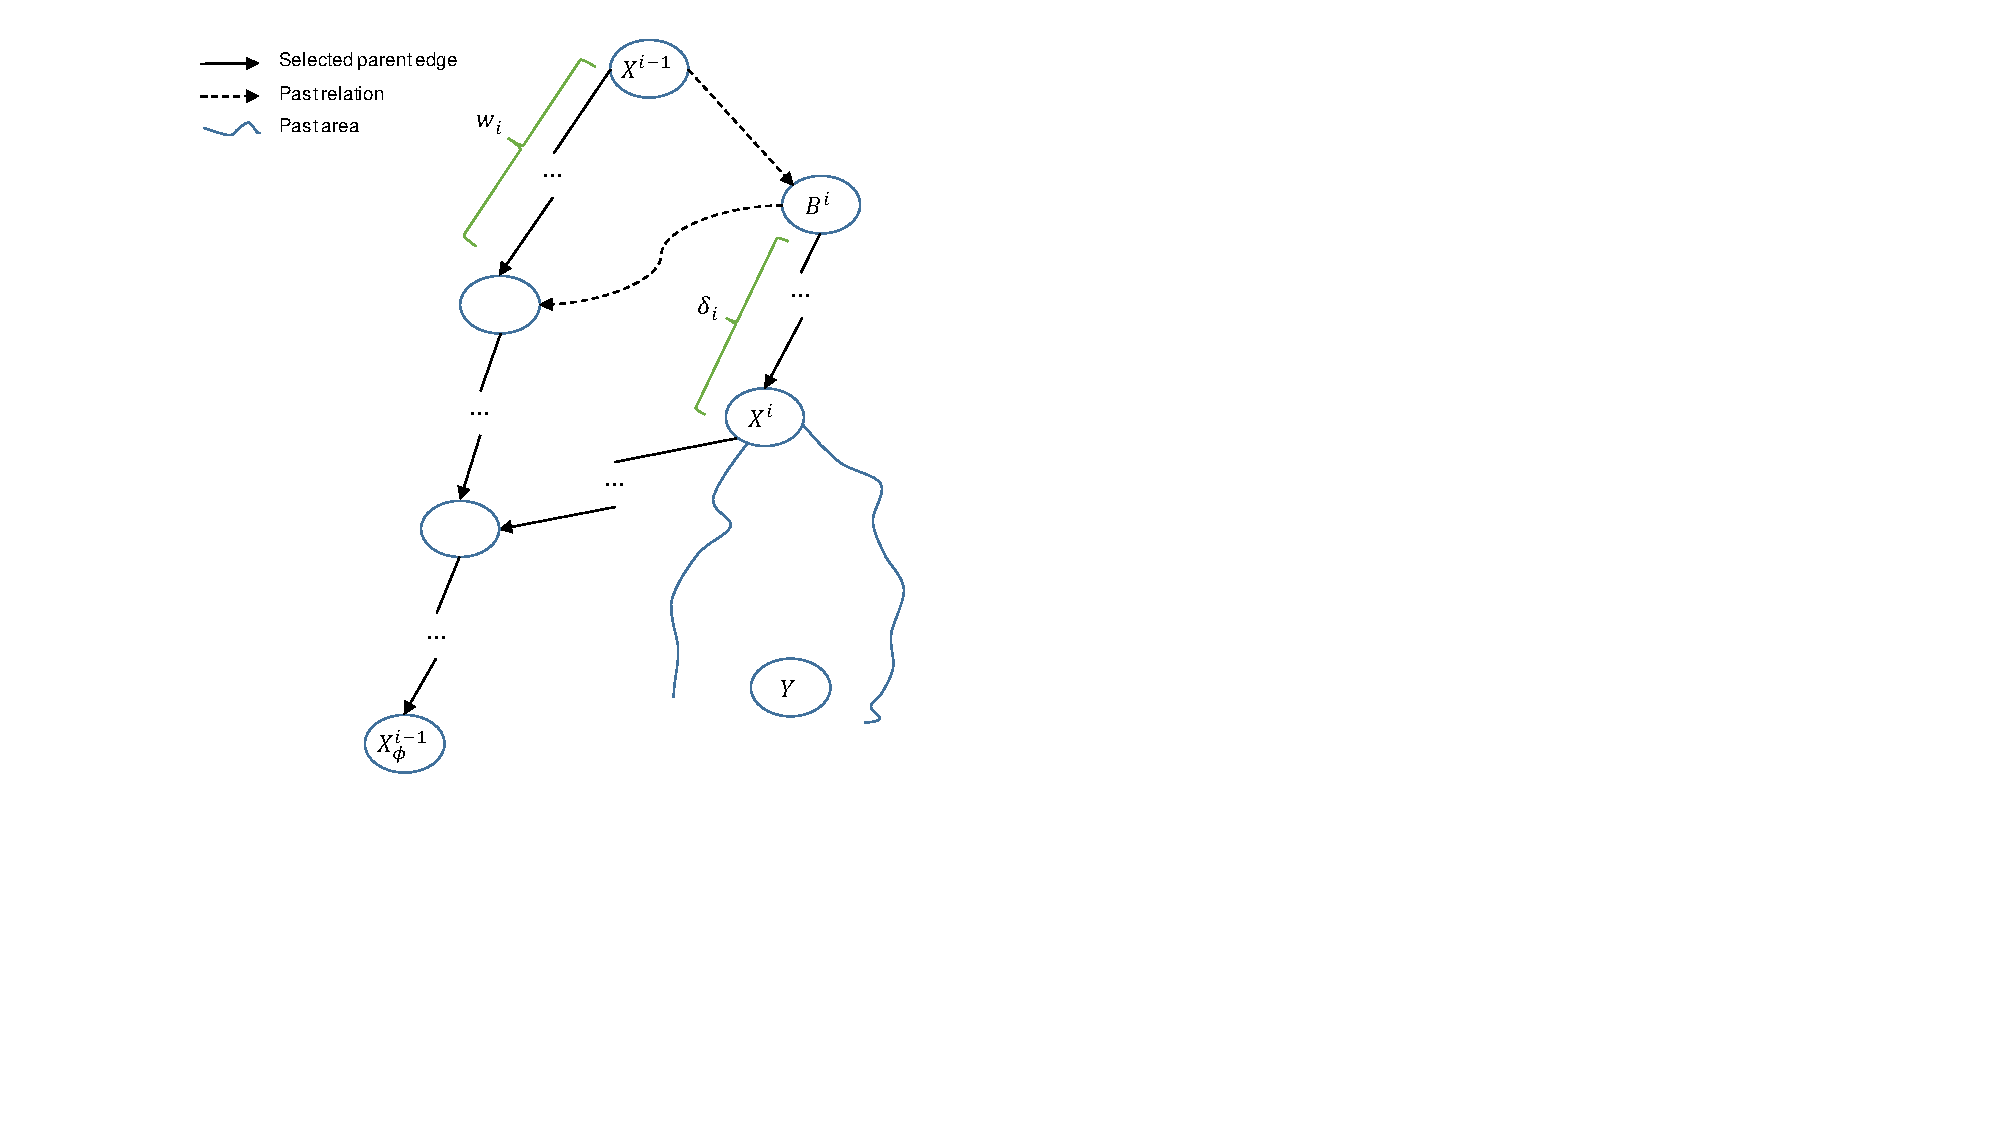
\includegraphics[width=0.75\textwidth, trim={3cm 5.5cm 18cm 0.5cm}, clip]{Pruning-Proof-Illustration.pdf}
        \caption{Illustration of induction variables.}
        \label{fig:induction}
    \end{figure}

    We now define a sequence of merging blocks $X = X^0,\ldots,X^m$, in the following way: 
    
    \begin{itemize}
        \item Given $X^{i-1}$, select a block $B^i \in Y.Future \cap X^{i-1}.Blues \cap X^{i-1}_\phi.Subtree $. Such a block must exist by induction hypothesis.
        % \item Since $Y \in B^i.Past$
        \item Select $X^{i}$ to be a block $\in B^i.\overline{C}hain$ s.t. $Y \in X^{i}.MergeSet$. Such a block must be unique if it exists. See Figure \ref{fig:induction} for an illustration. 
        \item If no such merging block exists, set $m = i-1$ and halt the process. This can only happen if $Y \in B^i.Chain$.
    \end{itemize}
    
    We now define counting measures for the process. Let 
    % $w_i$ be a minimal integer satisfying that $$X^{i-1}_{w_i} = \max X^{i-1}.Chain \cap B^i.Past;$$ 
    $w_i = \score{X^{i-1}} - \score{\max X^{i-1}.Chain \cap B^i.Past};$
    and denote $\delta_{i} = |B^{i}.Chain \setminus X^i.Chain|.$ 
    Note that $w_0, \delta_0$ are undefined and that $\delta_i = 0$ \emph{iff} $B^i = X^{i}$. See Figure \ref{fig:induction}.
    
    \begin{claim} \label{claim:freeload_dist}
        $$\comma{\forall i \in [1, \dots, m]}{w_i \le 4k + 1}$$ 
    \end{claim}
    \begin{proof}
        This follows from blueness of $B^i$ and from an argument similar to that of GHOSTDAG's \cite{sompolinsky2018phantom} freeloader bound ($B^i$ being a block freeloaded by $X^{i-1}$). 
        % Note that also without the freeloader bound, the $4k$ term can be easily replaced by $k^2$.
    \end{proof}
    
    \begin{claim} \label{claim:mergeset_lim}
        $$m + \sum_{i=1}^m \delta_i < \ell$$
    \end{claim}
    \begin{proof}
        Let $\Delta_i$ denote the set $B^{i}.\overline{C}hain \setminus X^{i}.Chain$. It needs to be shown that $\forall i \in [1, \dots, m], \Delta_i$ are disjoint subsets of $X.MergeSet \setminus \{Y\}$ which has size $< \ell$ by \ref{inv_merge}. 
        
        The subset property follows easily from the fact that all blocks in $\Delta_i$ are in $Y.Future \cap X.Past$. Assume that there exists a block $B \in Y.Future \cap X.Past, \notin X.MergeSet$, so $B, Y \in X.SelectedParent.Past$ which contradicts minimality of $X$. 
        The disjoint property follows directly from the inductive selection process.  
        Noting that $|\Delta_i| = \delta_i + 1$ gives the desired result.
    \end{proof}
    
    \begin{claim} \label{claim:score_dist}
        $$\score{X^m} > \score{F} - 4 \ell k$$
    \end{claim}
    
    \begin{proof}
        By definition of $w_i$ we have that
        % know that $X^{i-1}_{w_i} \in B^i.Past$, so 
        $\score{X^{i-1}} - w_i < \score{B^i}$. 
        Additionally, noting that $X^i \in B^i.\overline{C}hain$ and that each chain block can add at most $k+1$ blue blocks, we get that $\score{B^i} \le \score{X^{i}} + \delta_{i} \bigl(k+1\bigr)$.
        
        Reorganizing terms, we obtain a bound on the score distance between two consecutive merging blocks $$\score{X^{i-1}} - \score{X^{i}} < w_i + \delta_{i} \bigl(k+1\bigr);$$  
        
        Summing up this inequality over $i=1, \dots, m$ and using Claims \ref{claim:freeload_dist}, \ref{claim:mergeset_lim}, we get $\score{X^0} - \score{X^m} < m 4 k + \sum_{i=1}^m \delta_i (k+1) \le 4 \ell k$, where the last inequality holds since $k > 0$. The desired result follows since $F \in X^0.Past$, so $ \score{F} < \score{X^0}$.
    \end{proof}
    
    \begin{claim} \label{claim:finality_violated}
        $$\comma{\forall i \in [0, \dots, m]}{P \in X^i_\phi.Chain}$$
    \end{claim}
    
    \begin{proof}
        By induction on $i$. 
        
        \emph{Basis:} For $i=0, X = X^0$, the claim follows immediately since $ P, X_\phi \in X.Chain$ and $\score{X_\phi} > \score{P}$.  
        
        \emph{Inductive step:} 
        Assume that $P \in X^{i-1}_\phi.Chain$. We will now show that $P \in X^{i}_\phi.Chain$.
        By definition of $B^i$ we have that $X^{i-1}_\phi \in B^i.Chain$. The selection process also implies that $X^{i}_\phi, X^{i} \in B^i.Chain$.
        Combining with the induction hypothesis we get that $P, X^{i}_\phi \in B^i.Chain$. Since both blocks share a chain, it remains to show that $\score{P} < \score{X^{i}_\phi}$. 
        Following Claim \ref{claim:score_dist} and noting that $X^m \in X^i.Past$, we get that $\score{X^i} > \score{F} - 4 \ell k$. Combining with Corollary \ref{corollary:depth_bounds} over $X^i, \phi$ we have $$\score{X^i_\phi} > \score{F} - 4 \ell k - \phi - k - 1.$$ On the other hand, by plugging $\virt, \pi, \phi$ into Corollary \ref{corollary:depth_relation}, we get that $$\score{P} < \score{F} - 4 \ell k - \phi - k - 1;$$ so $\score{P} < \score{X^{i}_\phi}$. 
        
        
    \end{proof}
    
    \emph{Conclusion:} From Claim \ref{claim:finality_violated} it follows that $\forall i \in [0, \dots, m], Y \in X^i_\phi.Anticone$. To see this, note that $Y \in X^i_\phi.Future$ would imply that $Y \in P.Future$, which is a contradiction, and that $Y \in X^i_\phi.Past$ contradicts $Y \in X^i.MergeSet$. This justifies the induction hypothesis that $B^{i+1}$ must exist $\forall i \in [0, \dots, m]$, otherwise violating \ref{inv_fin}, \ref{inv_inh}. 
    Specifically, it must be assumed that $B^{m+1} \ne Y$ exists, where by definition $X^m_\phi \in B^{m+1}.Chain$. However by halting of the process it follows that $Y \in B^{m+1}.Chain$. Since $Y \in X^m_\phi.Anticone$, $Y,  X^m_\phi$ cannot share a chain, thus leading to a contradiction. 
    
\end{proof}

From this follows that it is secure to implement the following:

\begin{rule2} 
    \hfill
    \begin{itemize}
        \item All blocks in $P.Past$ can be pruned, and
        % \item If when $B$ was discovered it held that $B\notin P.Future$, then $B$ can be discarded.
        % TODO: should be: 
        \item For block $B$, if it holds that $B\notin P.Future$ and $B\notin \virt.Past$ (that is, $B$ violates finality rules of $\virt$), then $B$ can be discarded 
        % (in other words -- $P.Anticone$ is a final set)
    \end{itemize}
\end{rule2}

\bibliographystyle{plain}
\bibliography{prunality}

\end{document}